\documentclass[11pt,a4paper]{article}

% Pacotes essenciais
\usepackage[utf8]{inputenc}
\usepackage[T1]{fontenc}
\usepackage{lmodern}
\usepackage[portuguese]{babel}
\usepackage{graphicx}
\usepackage{amsmath}
\usepackage{amsfonts}
\usepackage{amssymb}
\usepackage{float}
\usepackage{caption}
\usepackage{subcaption}
\usepackage{xcolor}
\usepackage{colortbl}
\usepackage{fancyhdr}
\usepackage{geometry}
\usepackage{titlesec}
\usepackage{lipsum}
\usepackage{booktabs}
\usepackage{array}
\usepackage{enumitem}
\usepackage{tikz}
\usetikzlibrary{shapes.geometric}
\usepackage[hidelinks]{hyperref}

% Definição das cores
\definecolor{headercolor}{HTML}{b11116}
\definecolor{secondarycolor}{HTML}{3a5461}

% Configuração da página
\geometry{
    a4paper,
    top=2.8cm,
    bottom=2.5cm,
    left=2.5cm,
    right=2.5cm,
    headheight=1.2cm,
    headsep=0.5cm
}

% Configuração do cabeçalho
\pagestyle{fancy}
\fancyhf{}
\renewcommand{\headrulewidth}{0pt}
\renewcommand{\footrulewidth}{0.5pt}

\fancyhead[L]{%
    \begin{tikzpicture}[remember picture, overlay]
        \fill[headercolor] (current page.north west) rectangle ([yshift=-1.2cm]current page.north east);
        \node[anchor=west, inner sep=0pt] at ([xshift=1cm, yshift=-0.6cm]current page.north west) 
            {
\includegraphics[height=0.8cm]{imgs/base/fatec-rgt.png}};
        \node[anchor=east, inner sep=0pt] at ([xshift=-1cm, yshift=-0.6cm]current page.north east) 
            {
\includegraphics[height=0.9cm]{imgs/base/cps-logo.png}};
        \node[anchor=east, inner sep=0pt] at ([xshift=-2.8cm, yshift=-0.6cm]current page.north east) 
            {
\includegraphics[height=1.05cm]{imgs/base/governo-sp-secretaria-logo.png}};
    \end{tikzpicture}
}

\fancyfoot[L]{\footnotesize\textcolor{secondarycolor}{Faculdade de Tecnologia do Estado de São Paulo\\ fatecregistro.cps.sp.gov.br}}
\fancyfoot[R]{\thepage}

% Configuração dos títulos das seções
\titleformat{\section}
    {\normalfont\large\bfseries\color{secondarycolor}}
    {\thesection}{1em}{}

\titleformat{\subsection}
    {\normalfont\normalsize\bfseries\color{secondarycolor}}
    {\thesubsection}{1em}{}

\begin{document}

% ===== CAPA =====
\begin{titlepage}
    \centering
    
    % Logos no topo
    \begin{tikzpicture}[remember picture, overlay]
        \fill[headercolor] (current page.north west) rectangle ([yshift=-1.2cm]current page.north east);
        \node[anchor=west, inner sep=0pt] at ([xshift=1cm, yshift=-0.6cm]current page.north west) 
            {
\includegraphics[height=0.8cm]{imgs/base/fatec-rgt.png}};
        \node[anchor=east, inner sep=0pt] at ([xshift=-1cm, yshift=-0.6cm]current page.north east) 
            {
\includegraphics[height=0.9cm]{imgs/base/cps-logo.png}};
        \node[anchor=east, inner sep=0pt] at ([xshift=-2.8cm, yshift=-0.6cm]current page.north east) 
            {
\includegraphics[height=1.05cm]{imgs/base/governo-sp-secretaria-logo.png}};
    \end{tikzpicture}
    
    \vspace*{3.5cm}
    
    % Nome da faculdade
    {\normalsize FACULDADE DE TECNOLOGIA DO ESTADO DE SÃO PAULO\par}
    \vspace{0.5cm}
    
    % Curso
    {\normalsize DESENVOLVIMENTO DE SOFTWARE MULTIPLATAFORMA\par}
    
    \vspace{4cm}
    
    % Artefatos do Projeto de Software
    {\normalsize ARTEFATOS DO PROJETO DE SOFTWARE\par}
    
    \vspace{0.3cm}
    
    % Nome do projeto
    {\normalsize \textbf{CLASSIFICAÇÃO DE MANGANÊS E COBRE NA FOLHA DA MEXERICA,\
    ORIENTADO POR REDES NEURAIS}\par}
    
    \vspace{3cm}
    
    % Autores
    {\normalsize
    Amanda Vithória Alves Freitas\\
    Juliano Lopes Rodrigues Sales\\
    Lucas Gomes Fagundes\\
    Valéria de Freitas
    }
    
    \vfill
    
    % Rodapé
    {\small Registro -- SP\\
    2026}
    
\end{titlepage}

% Força o cabeçalho em todas as páginas
\pagestyle{fancy}

% ===== SUMÁRIO =====
\tableofcontents
\newpage

% ===== CANVAS =====
\section{CANVAS: Modelo de Negócio e Estratégia}

O Business Model Canvas é uma ferramenta de modelagem estratégica que permite descrever, analisar e
projetar o modelo de negócio de forma clara e objetiva. O Canvas do projeto de classificação de manganês e cobre na folha da mexerica contempla os
principais blocos de valor do sistema, focado na análise de deficiências nutricionais em folhas de mexerica.

\medskip
\noindent\textbf{Proposta de Valor}\\
O sistema ajuda agricultores a identificarem deficiências de manganês e cobre na folha da mexerica, oferecendo
análises automatizadas por meio de imagens e inteligência artificial.

\medskip
\noindent\textbf{Segmento de Mercado}\\
O público-alvo são agricultores de mexerica do Vale do Ribeira, com foco em produtores rurais, horticultores e
outros interessados na melhoria da produtividade agrícola.

\medskip
\noindent\textbf{Relacionamento com o Cliente}\\
O relacionamento será realizado por WhatsApp, aplicativo móvel e site institucional, com feedback automatizado
de análises por meio de gráficos e mapas.

\medskip
\noindent\textbf{Canais}\\
A divulgação e acesso ao sistema ocorrerão via secretarias de agricultura municipais, site, e-mail e WhatsApp,
fortalecendo a comunicação direta com o público-alvo.

\medskip
\noindent\textbf{Atividades-Chave}\\
As principais atividades são identificar deficiências nutricionais, oferecer suporte técnico e manter o sistema.

\medskip
\noindent\textbf{Recursos-Chave}\\
O sistema depende de equipe técnica, hospedagem para site e banco de dados, e infraestrutura de análise de imagens.

\medskip
\noindent\textbf{Parcerias-Chave}\\
As parcerias envolvem associações de fazendeiros, secretarias de agricultura e participação em feiras do setor.

\medskip
\noindent\textbf{Estrutura de Custos}\\
Inclui manutenção de equipamentos, aluguel de espaço físico, compra de materiais e custos de servidores.

\medskip
\noindent\textbf{Fontes de Renda}\\
A monetização pode ocorrer por meio de aluguel do sistema, cobrança por equipamentos e serviços de instalação e manutenção.

\begin{figure}[H]
\centering
\caption{Modelo de Negócios Canvas}
\label{fig:Canvas}
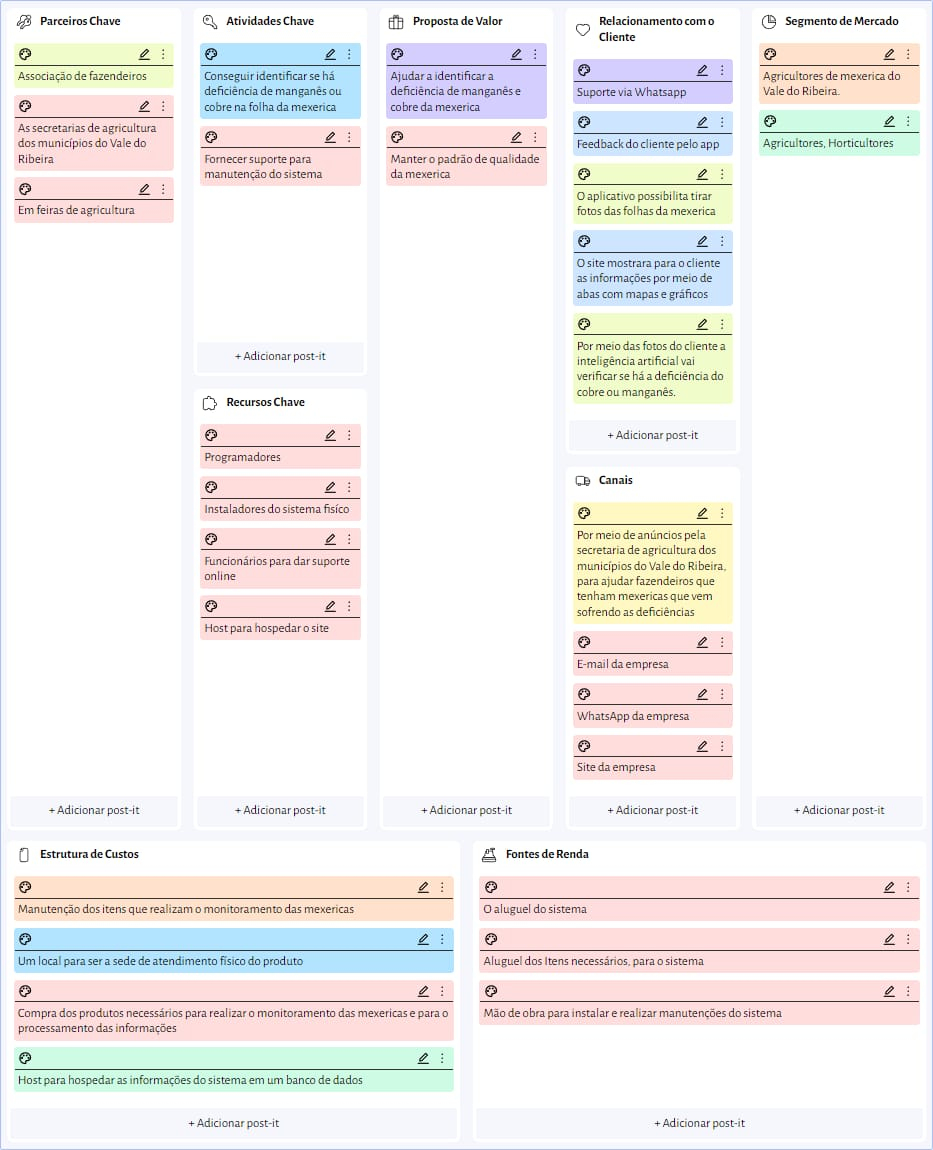
\includegraphics[width=0.8\textwidth]{imgs/Canvas.jpeg}
\end{figure}

\medskip

% ===== SWOT =====
\section{SWOT: Análise Estratégica}

A Análise SWOT (Strengths, Weaknesses, Opportunities, Threats) ou FOFA (Forças, Oportunidades, Fraquezas e Ameaças) \cite{oliveira2023} é uma ferramenta fundamental para planejamento estratégico\footnote{A análise SWOT foi criada na década de 1960 por Albert Humphrey no Stanford Research Institute.} que permite identificar fatores internos e externos que impactam o projeto. A análise SWOT foi realizada com o objetivo de compreender os principais pontos fortes, fracos, oportunidades e ameaças relacionadas ao projeto de classificação de manganês e cobre na folha da mexerica.

\subsection{Matriz SWOT}

A matriz SWOT do projeto está apresentada na Tabela~\ref{tab:swot}, organizando os fatores internos (forças e fraquezas) e externos (oportunidades e ameaças).

\begin{table}[H]
\centering
\caption{Análise SWOT do Projeto}
\label{tab:swot}
\begin{tabular}{|p{7.2cm}|p{7.2cm}|}
\hline
\multicolumn{2}{|c|}{\cellcolor{secondarycolor!20}\textbf{FATORES INTERNOS}} \\
\hline
\textbf{FORÇAS (Strengths)} & \textbf{FRAQUEZAS (Weaknesses)} \\
\hline
\begin{minipage}[t]{7cm}
\begin{itemize}[left=0pt]
  \item É alinhado com iniciativas sustentáveis.
  \item Melhora a eficiência e rapidez no diagnóstico de doenças.
  \item Reduz o risco de pés de mexerica ainda saudáveis.
  \item Reduz o desperdício de alimentos saudáveis.
  \item É alinhado com os objetivos da ODS.
\end{itemize}
\end{minipage}
&
\begin{minipage}[t]{7cm}
\begin{itemize}[left=0pt]
  \item Poucos estudos na área envolvendo plantas cítricas.
  \item O treinamento do modelo de IA depende de um grande banco de dados.
  \item O diagnóstico depende da qualidade da imagem.
  \item Dificuldade de acesso à internet por parte dos produtores.
\end{itemize}
\end{minipage}
\\
\hline
\multicolumn{2}{|c|}{\cellcolor{secondarycolor!20}\textbf{FATORES EXTERNOS}} \\
\hline
\textbf{OPORTUNIDADES (Opportunities)} & \textbf{AMEAÇAS (Threats)} \\
\hline
\begin{minipage}[t]{7cm}
\begin{itemize}[left=0pt]
  \item Expandir para outras deficiências como: zinco, ferro etc.
  \item Parcerias com empresas, cooperativas e universidades para divulgar o produto.
  \item Crescente demanda por agricultura de precisão.
\end{itemize}
\end{minipage}
&
\begin{minipage}[t]{7cm}
\begin{itemize}[left=0pt]
  \item Resistência por parte dos produtores tradicionais.
  \item Concorrência com outras soluções, como drones, por exemplo.
\end{itemize}
\end{minipage}
\\
\hline
\end{tabular}
\end{table}

\medskip
Esse tipo de avaliação permite identificar elementos que podem impactar diretamente o sucesso do sistema, além de apontar caminhos para melhorias contínuas e decisões estratégicas.

\subsection{Recomendações Estratégicas}

Com base na análise SWOT, as principais estratégias devem focar em:
\begin{itemize}
    \item \textbf{Forças + Oportunidades:} Posicionar a solução no mercado de agricultura de precisão, destacando o alinhamento com práticas sustentáveis e os Objetivos de Desenvolvimento Sustentável (ODS), e buscar parcerias com cooperativas e universidades para ampliar a divulgação.
    \item \textbf{Forças + Ameaças:} Reforçar a proposta de valor frente à concorrência (como drones), enfatizando o diagnóstico rápido por imagem da folha, a redução de desperdício e a preservação de pés saudáveis de mexerica.
    \item \textbf{Fraquezas + Oportunidades:} Estabelecer parcerias com universidades e cooperativas para ampliar o banco de dados de treinamento da IA e validar cientificamente a solução em plantas cítricas, aproveitando a demanda por agricultura de precisão.
    \item \textbf{Fraquezas + Ameaças:} Mitigar a resistência dos produtores tradicionais com materiais de capacitação sobre captura de imagens e uso do sistema, e planejar funcionalidades que reduzam a dependência de conectividade contínua.
\end{itemize}

% ===== UX/UI =====
\section{UX/UI: Design de Interface e Experiência do Usuário}

Esta seção apresenta os principais protótipos de interface do sistema, incluindo as versões web e mobile,
com foco em usabilidade e navegação.

\subsection{Interface Web}

A interface web apresenta telas de login, histórico, resultados e mapa, todas alinhadas ao fluxo de
navegação do usuário.

\begin{figure}[H]
\centering
\caption{Protótipo Interface Web - Tela de Login}
\label{fig:interface-web-tela-login}

\includegraphics[width=0.8\textwidth]{imgs/TelaLogin.png}
\end{figure}

A tela de login permite o acesso de usuários cadastrados, garantindo segurança e controle de autenticação.

\begin{figure}[H]
\centering
\caption{Protótipo Interface Web - Tela de Histórico}
\label{fig:interface-web-tela-historico}

\includegraphics[width=0.8\textwidth]{imgs/TelaHistorico-1.png}
\end{figure}

A tela de histórico apresenta registros anteriores de análises feitas em cada talhão, permitindo acompanhar a
evolução das deficiências identificadas.

\begin{figure}[H]
\centering
\caption{Protótipo Interface Web - Tela de Resultados}
\label{fig:interface-web-tela-resultados}

\includegraphics[width=0.8\textwidth]{imgs/TelaResultado.png}
\end{figure}

A tela de resultados exibe as análises feitas a partir das imagens enviadas, incluindo diagnósticos e relatórios de
forma clara.

\begin{figure}[H]
\centering
\caption{Protótipo Interface Web - Tela de Mapa}
\label{fig:interface-web-tela-mapa}

\includegraphics[width=0.8\textwidth]{imgs/TelaMapa.png}
\end{figure}

Nesta tela, o usuário visualiza os talhões de sua propriedade em um mapa interativo.

\subsection{Interface Mobile}

A interface mobile reproduz as principais funcionalidades da versão web, adaptada para telas menores e navegação
por toque.

\begin{figure}[H]
\centering
\caption{Protótipo Interface Mobile - Tela de Login}
\label{fig:interface-mobile-tela-login}

\includegraphics[width=0.4\textwidth]{imgs/MobileLogin.png}
\end{figure}

\begin{figure}[H]
\centering
\caption{Protótipo Interface Mobile - Tela de Início}
\label{fig:interface-mobile-tela-inicio}

\includegraphics[width=0.4\textwidth]{imgs/MobileInicio.png}
\end{figure}

\begin{figure}[H]
\centering
\caption{Protótipo Interface Mobile - Tela de Histórico}
\label{fig:interface-mobile-tela-historico-mobile}

\includegraphics[width=0.4\textwidth]{imgs/MobileHistorico.png}
\end{figure}

\begin{figure}[H]
\centering
\caption{Protótipo Interface Mobile - Tela de Resultados}
\label{fig:interface-mobile-tela-resultados-mobile}

\includegraphics[width=0.4\textwidth]{imgs/MobileResultado.png}
\end{figure}

\begin{figure}[H]
\centering
\caption{Protótipo Interface Mobile - Tela de Mapa}
\label{fig:interface-mobile-tela-mapa-mobile}

\includegraphics[width=0.4\textwidth]{imgs/MobileMapa.png}
\end{figure}

A versão mobile garante acesso prático e rápido às principais funcionalidades do sistema em dispositivos portáteis.

% ===== WEBSITE =====
\section{Website: Estrutura e Especificações Técnicas Web}

Esta seção apresenta as principais telas do sistema Web desenvolvidas em Node.js (Express + Sequelize)
com MySQL e EJS. A versão mostra a estrutura básica, a navegação entre páginas e o funcionamento do banco de dados.

\begin{figure}[H]
\centering
\caption{Interface Web - Tela de Login}
\label{fig:website-tela-login}
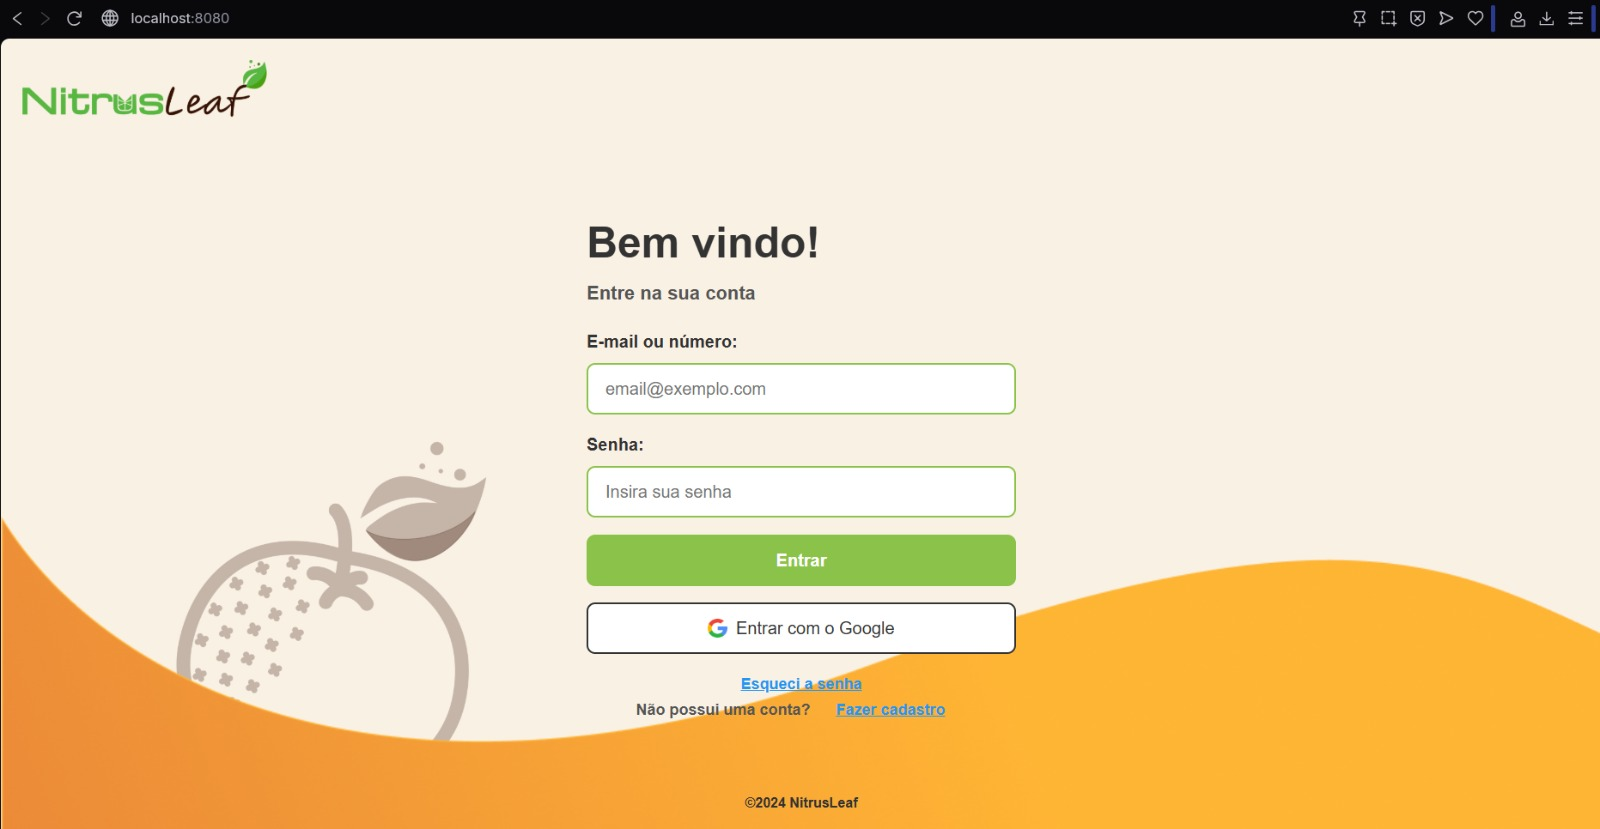
\includegraphics[width=0.8\textwidth]{imgs/AppLogin.png}
\end{figure}

A tela de login está fiel ao protótipo e implementa autenticação via middleware.

\begin{figure}[H]
\centering
\caption{Interface Web - Tela de Início}
\label{fig:website-tela-inicio}
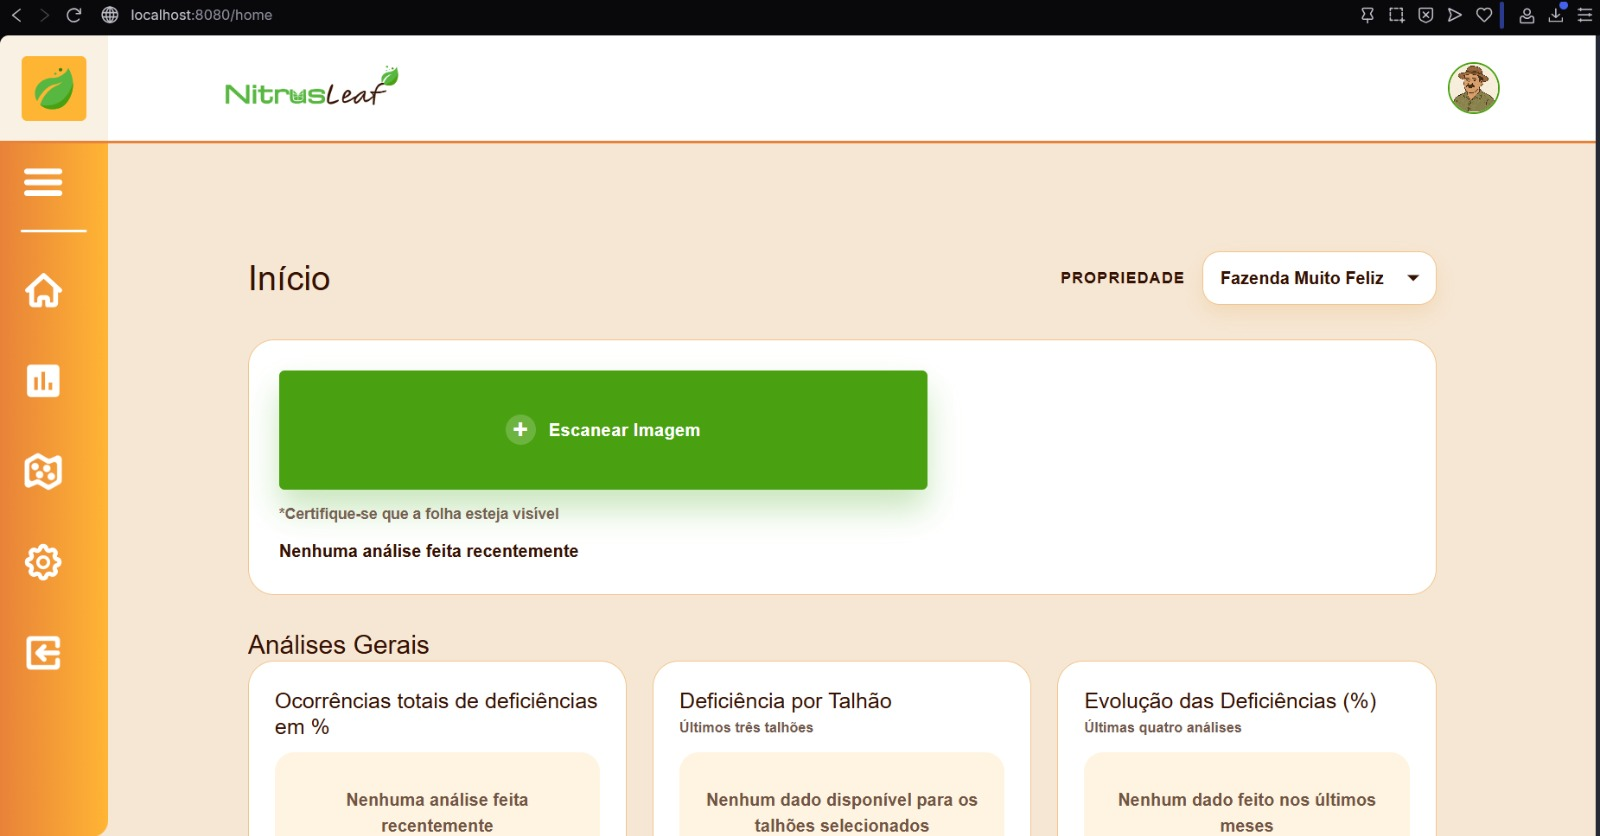
\includegraphics[width=0.8\textwidth]{imgs/AppInicio.jpeg}
\end{figure}

A tela de início é a primeira visão do usuário após o login.

\begin{figure}[H]
\centering
\caption{Interface Web - Tela de Resultados}
\label{fig:website-tela-resultados-app}
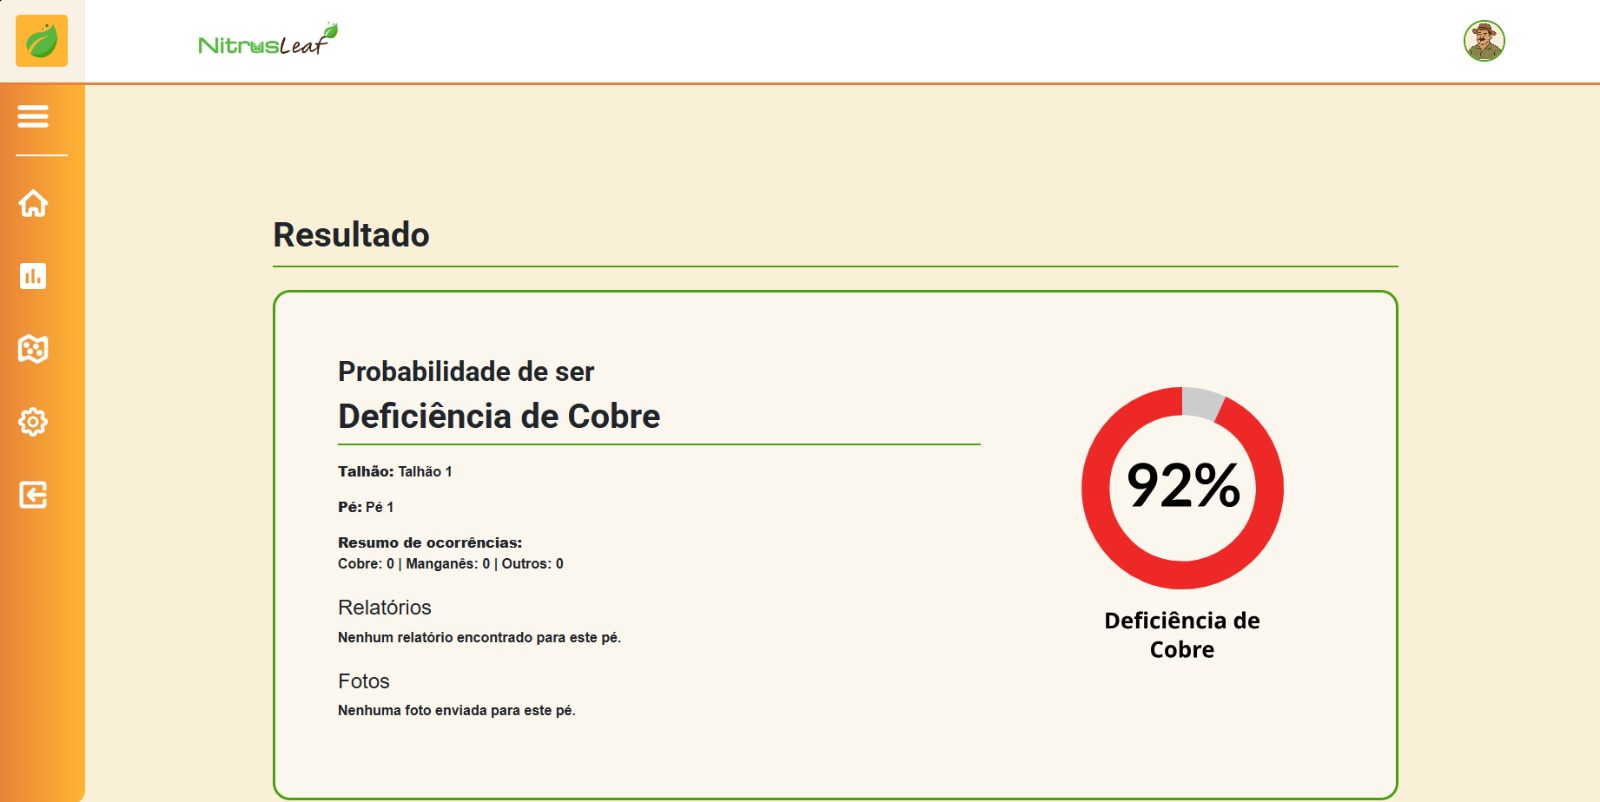
\includegraphics[width=0.8\textwidth]{imgs/AppResultado.jpeg}
\end{figure}

A tela de resultados exibe análises detalhadas das imagens enviadas.

\begin{figure}[H]
\centering
\caption{Interface Web - Tela de Histórico}
\label{fig:website-tela-historico-app}
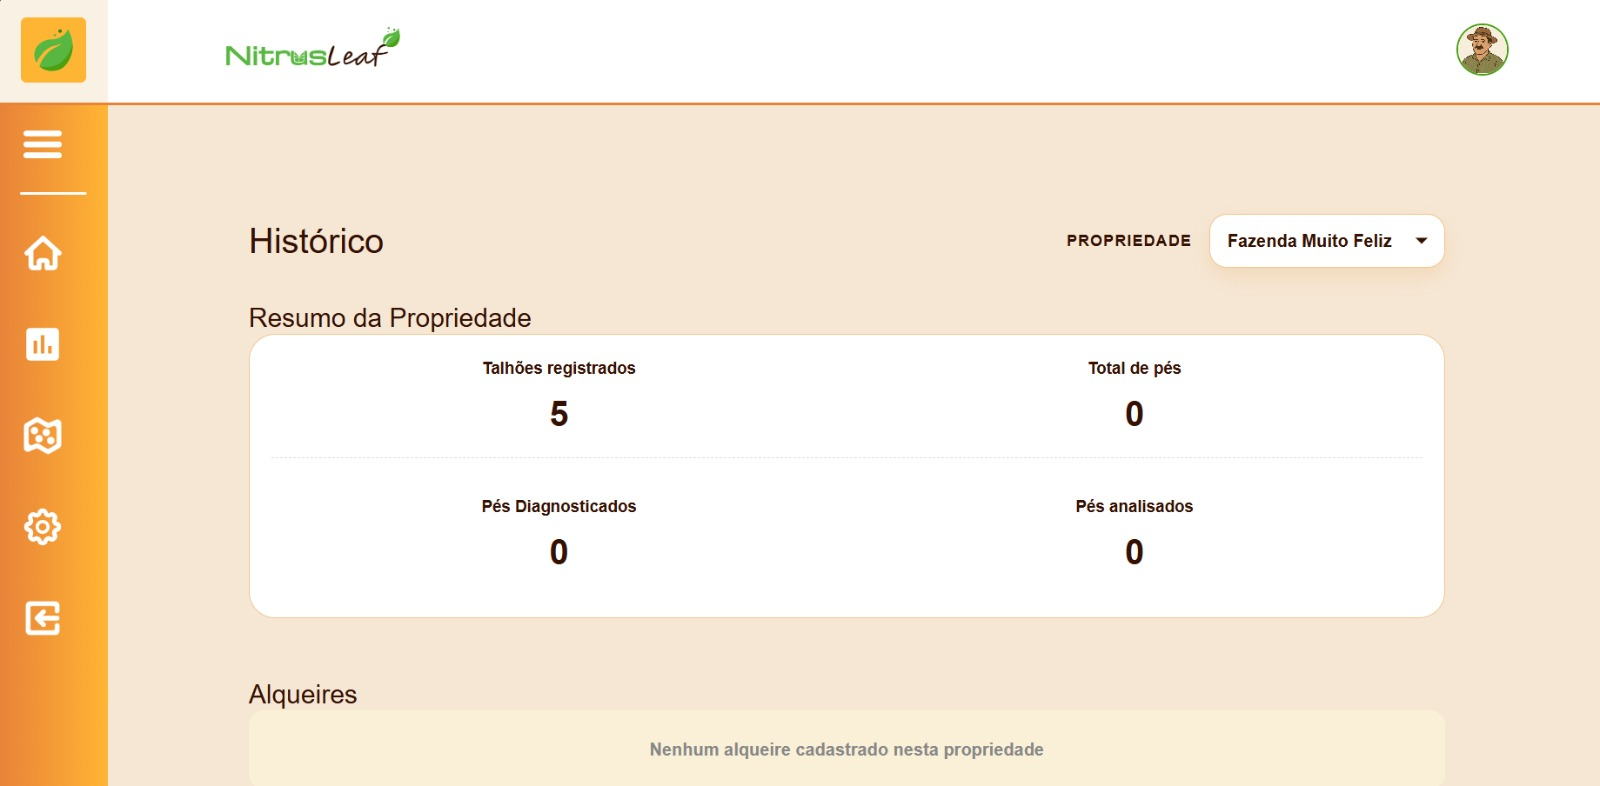
\includegraphics[width=0.8\textwidth]{imgs/AppHistorico.jpeg}
\end{figure}

A tela de histórico permite visualizar interações anteriores, acompanhando o fluxo.

\begin{figure}[H]
\centering
\caption{Interface Web - Tela de Mapa}
\label{fig:website-tela-mapa-app}
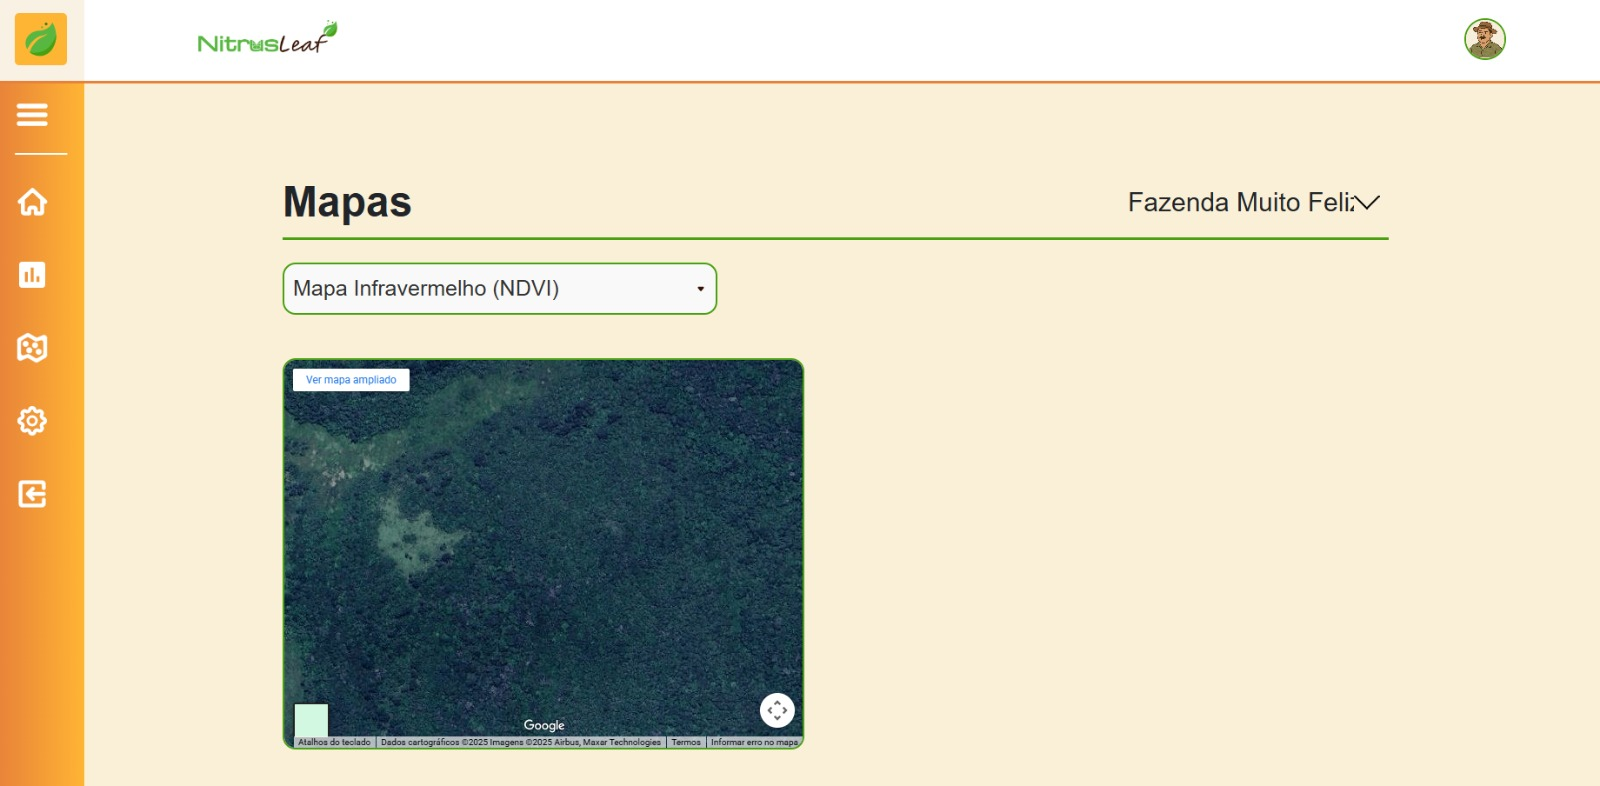
\includegraphics[width=0.8\textwidth]{imgs/AppMapa.jpeg}
\end{figure}

A tela de mapa permite visualizar a localização geográfica da propriedade analisada.

% ===== DIAGRAMAS UML =====
\section{Diagramas UML: Modelagem Visual do Sistema}

A modelagem UML permite representar visualmente a arquitetura e as interações do sistema.
A seguir, são apresentados os principais diagramas que suportam o projeto de classificação de manganês e cobre na folha da mexerica.

\subsection{Diagrama de Casos de Uso}

\noindent\textbf{Atores do Sistema:}
\begin{itemize}[itemsep=0.6em, topsep=0.3em, parsep=0pt]
    \item \textbf{Usuário (Cliente)}: acessa o sistema para realizar cadastro/login, consultar informações, criar/editar solicitações e acompanhar status.
    \item \textbf{Administrador}: gerencia cadastros, permissões, configurações gerais e monitora registros/relatórios.
    \item \textbf{Operador/Atendente}: valida dados enviados pelos usuários, aprova/reprova solicitações e atualiza status operacionais.
    \item \textbf{Sistema Externo (API/Integrações)}: provê dados de serviços de terceiros (ex.: pagamento, mapas, notificações).
\end{itemize}

\noindent\textbf{Casos de Uso do Sistema:}
\begin{itemize}[itemsep=0.6em, topsep=0.3em, parsep=0pt]
    \item \textbf{Autenticar Usuário}: cadastro, login e recuperação de senha.
    \item \textbf{Gerenciar Perfis}: editar dados pessoais, preferências e documentos.
    \item \textbf{Registrar Solicitação}: criar, editar e cancelar solicitações.
    \item \textbf{Acompanhar Status}: visualizar andamento, receber notificações e histórico.
    \item \textbf{Gerir Operações (Backoffice)}: triagem, aprovação e ajustes operacionais.
    \item \textbf{Relatórios e Auditoria}: visualizar métricas, exportar dados e rastrear logs.
    \item \textbf{Integrações}: consultar/enviar dados para APIs externas.
\end{itemize}

\begin{figure}[H]
\centering
\caption{Diagrama de Caso de Uso}
\label{fig:diagrama-caso-uso}
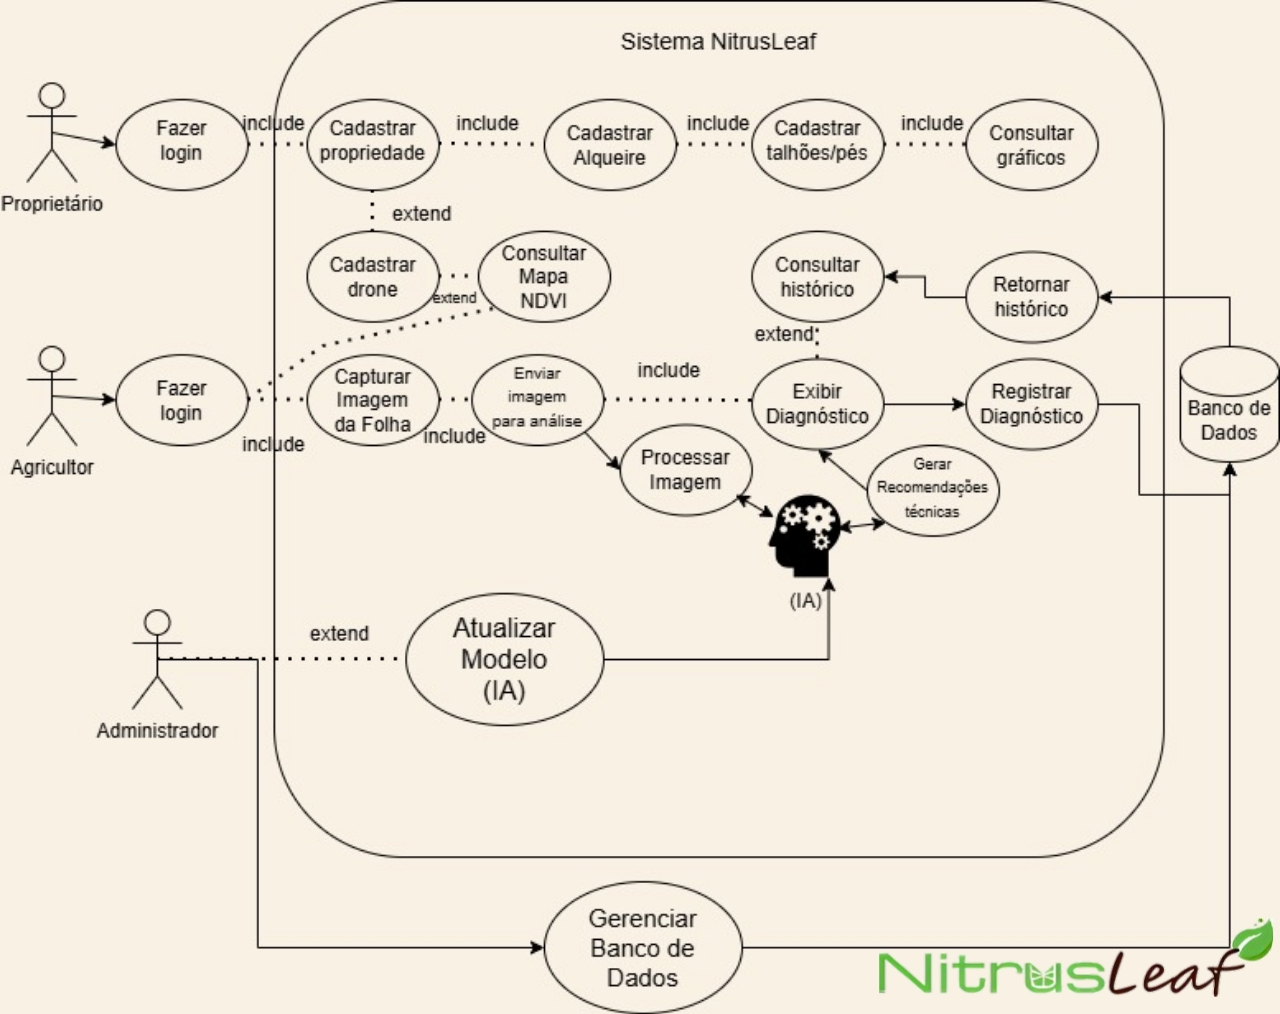
\includegraphics[width=0.8\textwidth]{imgs/DiagramaCasosDeUso.jpg}
\end{figure}

\subsection{Diagrama de Classe}

O diagrama de classes resume as principais entidades do sistema e seus relacionamentos.

\begin{itemize}[itemsep=0.6em, topsep=0.3em, parsep=0pt]
    \item \textbf{Propriedade}: cadastra e gerencia propriedades rurais vinculadas a um usuário.
    \item \textbf{Usuário}: mantém dados pessoais e de autenticação, suportando cadastro e login.
    \item \textbf{Talhão}: subárea da propriedade que guarda metadados e histórico de diagnósticos.
    \item \textbf{Diagnóstico}: registra análise por imagem, vínculo ao talhão e resultado do laudo.
    \item \textbf{ServidorNode}: faz a ponte do frontend com a API e encaminha requisições para processamento.
    \item \textbf{ProcessamentoPython}: executa classificação de imagens com CNN e atualiza o modelo.
    \item \textbf{BancoDeDados}: gerencia conexão e operações CRUD para persistência dos dados.
    \item \textbf{PainelAdmin}: área administrativa para gestão de usuários, modelos e monitoramento.
\end{itemize}

\begin{figure}[H]
\centering
\caption{Diagrama de Classe}
\label{fig:diagrama-classe}
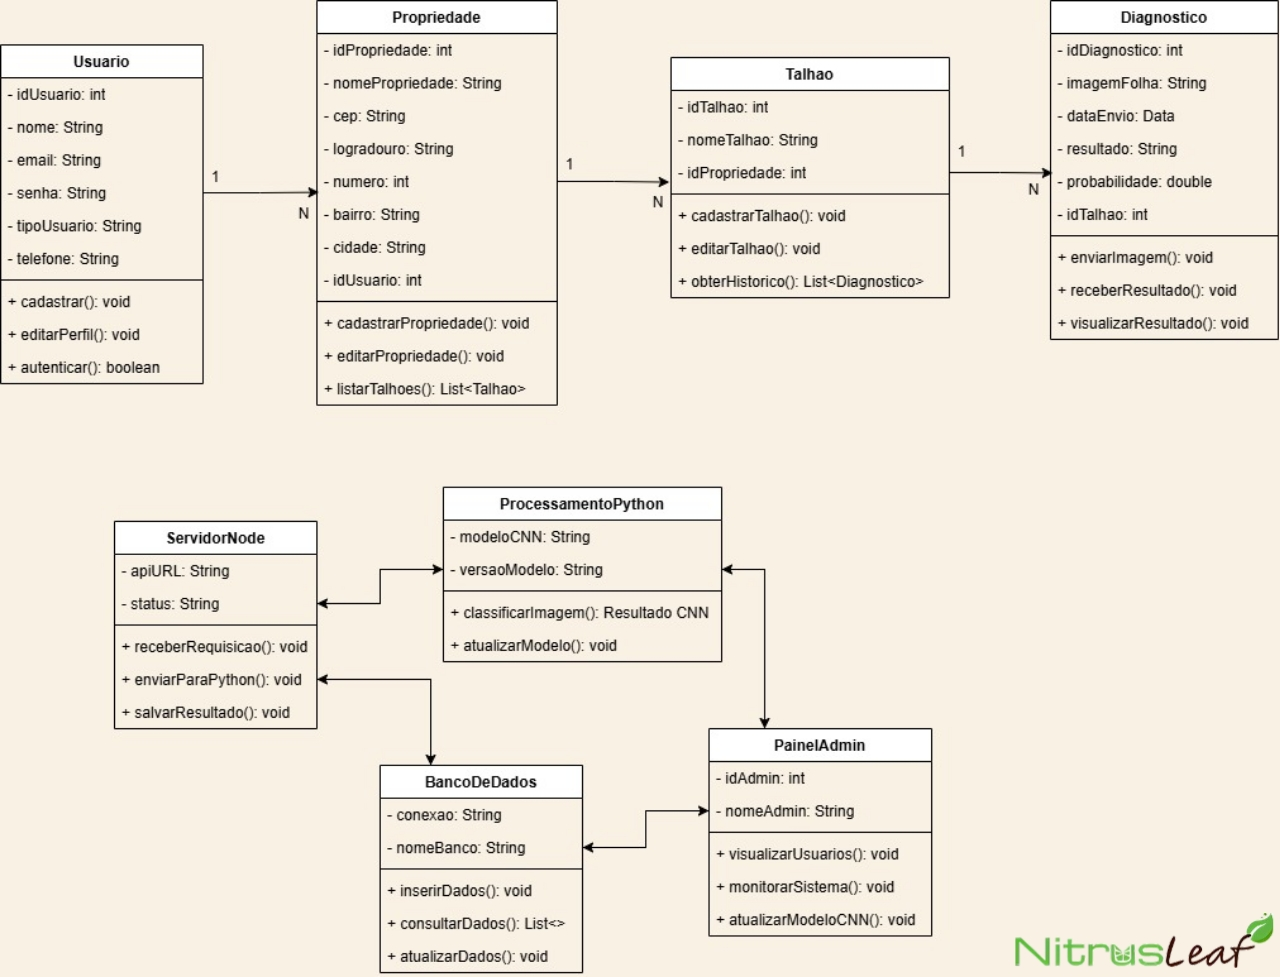
\includegraphics[width=0.8\textwidth]{imgs/DiagramaDeClasses.jpg}
\end{figure}

\subsection{Diagrama de Objetos}

O diagrama de objetos apresenta instâncias concretas e o fluxo de criação e vinculação entre elas.

\begin{figure}[H]
\centering
\caption{Diagrama de Objetos}
\label{fig:diagrama-objetos}
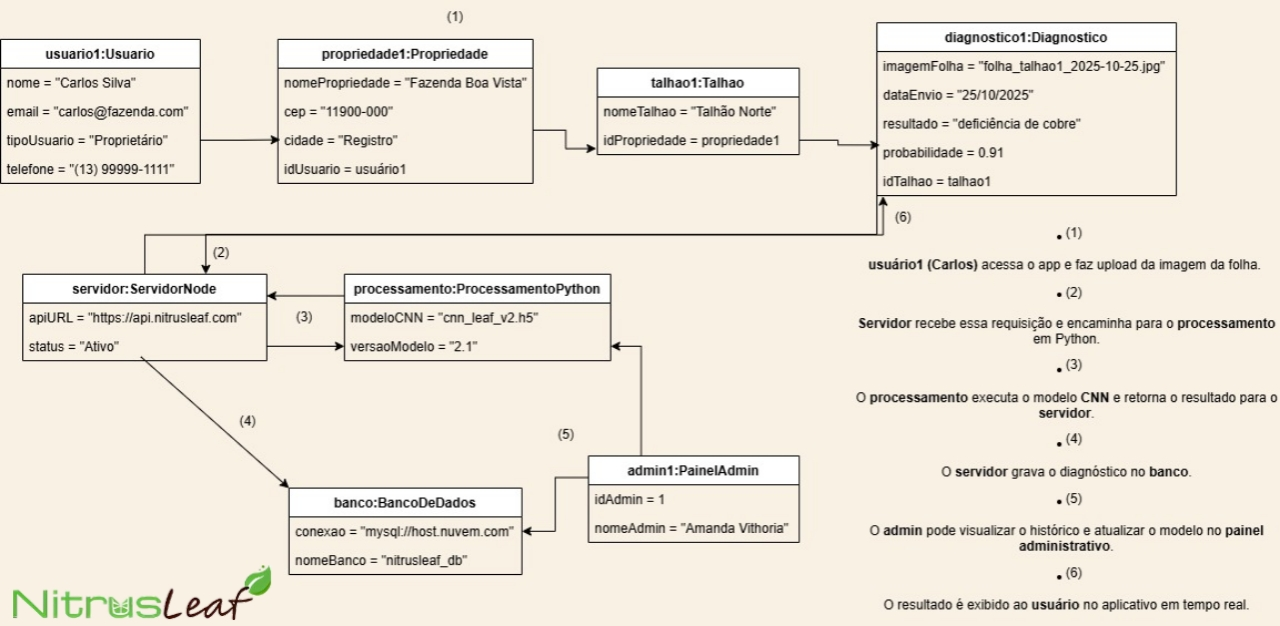
\includegraphics[width=0.8\textwidth]{imgs/DiagramaDeObjetos.jpg}
\end{figure}

\subsection{Diagrama Entidade–Relacionamento}

O diagrama Entidade–Relacionamento descreve a estrutura lógica do banco de dados,
com entidades como Usuários, Propriedades, Talhões, Pés, Fotos e Relatórios.

\begin{figure}[H]
\centering
\caption{Diagrama Entidade–Relacionamento}
\label{fig:diagrama-der}
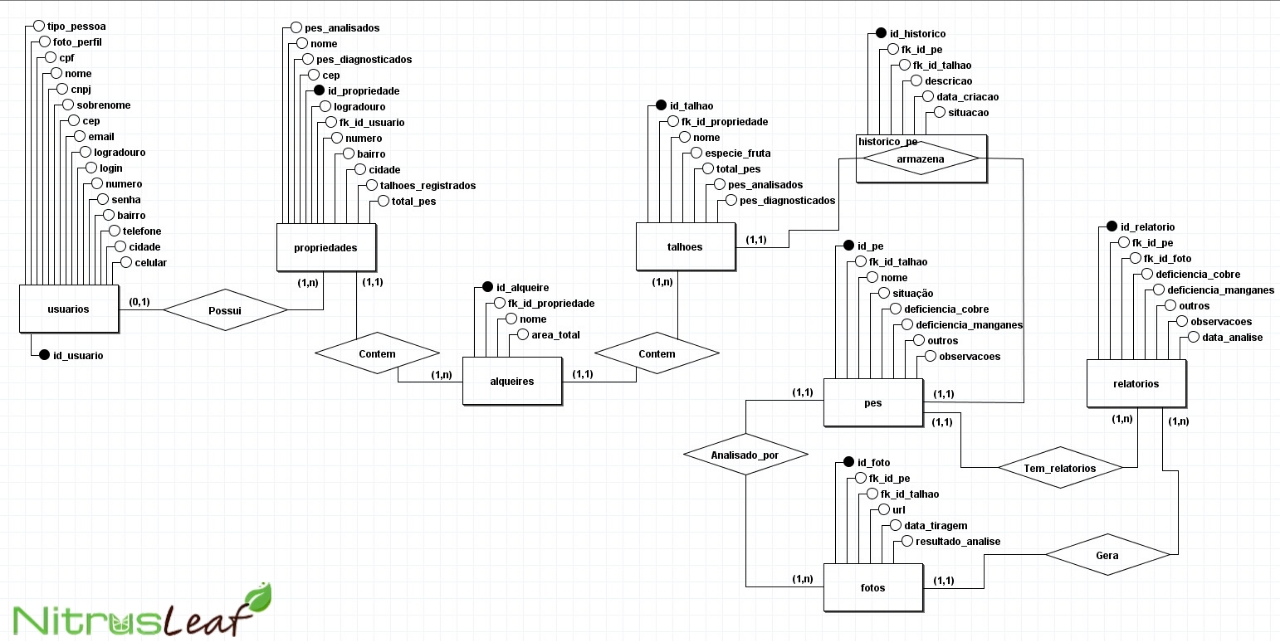
\includegraphics[width=0.9\textwidth]{imgs/DiagramaDER.jpg}
\end{figure}

\subsection{Diagrama Modelo Lógico}

O modelo lógico descreve a hierarquia dos dados e a ligação entre entidades do sistema.

\begin{figure}[H]
\centering
\caption{Diagrama Modelo Lógico}
\label{fig:diagrama-mer}
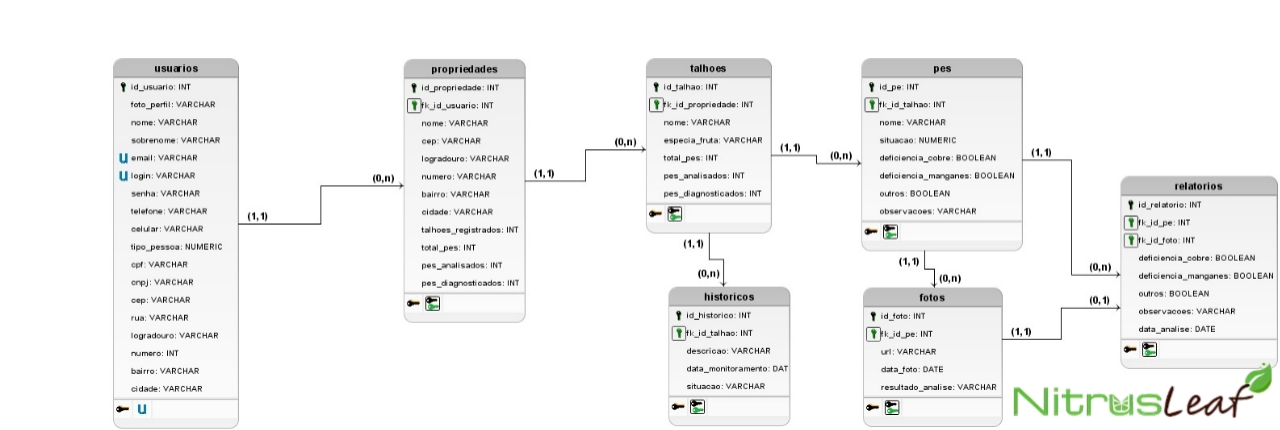
\includegraphics[width=0.9\textwidth]{imgs/DiagramaMER.jpg}
\end{figure}

% ===== DEVOPS =====
\section{DevOps: Infraestrutura, Automação e Práticas}

O conteúdo de DevOps ainda não está disponível para este projeto. Esta seção será preenchida
posteriormente quando as informações de pipeline, infraestrutura e automação estiverem definidas.

\newpage
\section*{Conclusão}

Este documento apresenta os artefatos do projeto \textbf{Classificação de Manganês e Cobre na Folha da Mexerica}, reunindo o planejamento estratégico, a análise SWOT, o design UX/UI, a especificação de website, os diagramas UML e o relatório de DevOps.

\newpage
\section*{Referências}
\addcontentsline{toc}{section}{Referências}
\begin{thebibliography}{1}
\bibitem{oliveira2023}
OLIVEIRA, P.; COSTA, M. Machine learning applications in dynamic systems.
\emph{IEEE Transactions on Systems, Man, and Cybernetics}, IEEE, v.~53, n.~8,
  p. 4567--4580, 2023.
\end{thebibliography}

\end{document}
